\documentclass[twoside]{book}

% Packages required by doxygen
\usepackage{fixltx2e}
\usepackage{calc}
\usepackage{doxygen}
\usepackage[export]{adjustbox} % also loads graphicx
\usepackage{graphicx}
\usepackage[utf8]{inputenc}
\usepackage{makeidx}
\usepackage{multicol}
\usepackage{multirow}
\PassOptionsToPackage{warn}{textcomp}
\usepackage{textcomp}
\usepackage[nointegrals]{wasysym}
\usepackage[table]{xcolor}

% Font selection
\usepackage[T1]{fontenc}
\usepackage[scaled=.90]{helvet}
\usepackage{courier}
\usepackage{amssymb}
\usepackage{sectsty}
\renewcommand{\familydefault}{\sfdefault}
\allsectionsfont{%
  \fontseries{bc}\selectfont%
  \color{darkgray}%
}
\renewcommand{\DoxyLabelFont}{%
  \fontseries{bc}\selectfont%
  \color{darkgray}%
}
\newcommand{\+}{\discretionary{\mbox{\scriptsize$\hookleftarrow$}}{}{}}

% Page & text layout
\usepackage{geometry}
\geometry{%
  a4paper,%
  top=2.5cm,%
  bottom=2.5cm,%
  left=2.5cm,%
  right=2.5cm%
}
\tolerance=750
\hfuzz=15pt
\hbadness=750
\setlength{\emergencystretch}{15pt}
\setlength{\parindent}{0cm}
\setlength{\parskip}{3ex plus 2ex minus 2ex}
\makeatletter
\renewcommand{\paragraph}{%
  \@startsection{paragraph}{4}{0ex}{-1.0ex}{1.0ex}{%
    \normalfont\normalsize\bfseries\SS@parafont%
  }%
}
\renewcommand{\subparagraph}{%
  \@startsection{subparagraph}{5}{0ex}{-1.0ex}{1.0ex}{%
    \normalfont\normalsize\bfseries\SS@subparafont%
  }%
}
\makeatother

% Headers & footers
\usepackage{fancyhdr}
\pagestyle{fancyplain}
\fancyhead[LE]{\fancyplain{}{\bfseries\thepage}}
\fancyhead[CE]{\fancyplain{}{}}
\fancyhead[RE]{\fancyplain{}{\bfseries\leftmark}}
\fancyhead[LO]{\fancyplain{}{\bfseries\rightmark}}
\fancyhead[CO]{\fancyplain{}{}}
\fancyhead[RO]{\fancyplain{}{\bfseries\thepage}}
\fancyfoot[LE]{\fancyplain{}{}}
\fancyfoot[CE]{\fancyplain{}{}}
\fancyfoot[RE]{\fancyplain{}{\bfseries\scriptsize Generated by Doxygen }}
\fancyfoot[LO]{\fancyplain{}{\bfseries\scriptsize Generated by Doxygen }}
\fancyfoot[CO]{\fancyplain{}{}}
\fancyfoot[RO]{\fancyplain{}{}}
\renewcommand{\footrulewidth}{0.4pt}
\renewcommand{\chaptermark}[1]{%
  \markboth{#1}{}%
}
\renewcommand{\sectionmark}[1]{%
  \markright{\thesection\ #1}%
}

% Indices & bibliography
\usepackage{natbib}
\usepackage[titles]{tocloft}
\setcounter{tocdepth}{3}
\setcounter{secnumdepth}{5}
\makeindex

% Hyperlinks (required, but should be loaded last)
\usepackage{ifpdf}
\ifpdf
  \usepackage[pdftex,pagebackref=true]{hyperref}
\else
  \usepackage[ps2pdf,pagebackref=true]{hyperref}
\fi
\hypersetup{%
  colorlinks=true,%
  linkcolor=blue,%
  citecolor=blue,%
  unicode%
}

% Custom commands
\newcommand{\clearemptydoublepage}{%
  \newpage{\pagestyle{empty}\cleardoublepage}%
}

\usepackage{caption}
\captionsetup{labelsep=space,justification=centering,font={bf},singlelinecheck=off,skip=4pt,position=top}

%===== C O N T E N T S =====

\begin{document}

% Titlepage & ToC
\hypersetup{pageanchor=false,
             bookmarksnumbered=true,
             pdfencoding=unicode
            }
\pagenumbering{alph}
\begin{titlepage}
\vspace*{7cm}
\begin{center}%
{\Large robot\+\_\+interface }\\
\vspace*{1cm}
{\large Generated by Doxygen 1.8.13}\\
\end{center}
\end{titlepage}
\clearemptydoublepage
\pagenumbering{roman}
\tableofcontents
\clearemptydoublepage
\pagenumbering{arabic}
\hypersetup{pageanchor=true}

%--- Begin generated contents ---
\chapter{robot\+\_\+interface}
\label{index}\hypertarget{index}{}R\+O\+S2 package to use robot native interface

\subsection*{Install}

Install dependency {\bfseries ur\+\_\+modern\+\_\+driver}\+:


\begin{DoxyCode}
git clone -b libur\_modern\_driver https://github.com/RoboticsYY/ur\_modern\_driver.git
cd ur\_modern\_driver/libur\_modern\_driver
mkdir build && cd build
cmake .. && sudo make install
\end{DoxyCode}


Install dependency {\bfseries ros2\+\_\+ur\+\_\+description}\+:


\begin{DoxyCode}
mkdir -p ~/ros2\_ws/src && cd ~/ros2\_ws/src
git clone https://github.com/RoboticsYY/ros2\_ur\_description.git
cd .. && colcon build
\end{DoxyCode}


Install {\bfseries robot\+\_\+interface}\+:

The installation should refer to the installation of {\bfseries ros2\+\_\+grasp\+\_\+library}.

\begin{quote}
Note\+: If error \char`\"{}fatal error\+: Eigen/\+Geometry\+: No such file or directory\char`\"{} persists during the compilation, please check the file path of \char`\"{}\+Eigen/\+Geometry\char`\"{}, if it locates at \char`\"{}/usr/include/eigen3/\+Eigen\char`\"{}, a work around is creating a soft link to \char`\"{}/usr/include/\+Eigen\char`\"{} as below\+: \end{quote}



\begin{DoxyCode}
ln -s /usr/include/eigen3/Eigen /usr/include/Eigen
\end{DoxyCode}


\subsection*{Launch}

Launch the UR robot control test executable\+:


\begin{DoxyCode}
ros2 launch robot\_interface ur\_test.launch.py move:=true
\end{DoxyCode}


Launch the Rivz2 display\+:


\begin{DoxyCode}
ros2 launch ur\_description view\_ur5\_ros2.launch.py
\end{DoxyCode}


\subsection*{Generate Document}


\begin{DoxyCode}
cd <path to root of ros2\_grasp\_library>/grasp\_utils/robot\_interface

doxygen Doxyfile
\end{DoxyCode}
 
\chapter{Hierarchical Index}
\section{Class Hierarchy}
This inheritance list is sorted roughly, but not completely, alphabetically\+:\begin{DoxyCompactList}
\item Node\begin{DoxyCompactList}
\item \contentsline{section}{Arm\+Control\+Base}{\pageref{classArmControlBase}}{}
\end{DoxyCompactList}
\item \contentsline{section}{Tcp\+Pose}{\pageref{structTcpPose}}{}
\end{DoxyCompactList}

\chapter{Class Index}
\section{Class List}
Here are the classes, structs, unions and interfaces with brief descriptions\+:\begin{DoxyCompactList}
\item\contentsline{section}{\hyperlink{classArmControlBase}{Arm\+Control\+Base} \\*Robot arm control interface }{\pageref{classArmControlBase}}{}
\item\contentsline{section}{\hyperlink{structTcpPose}{Tcp\+Pose} \\*Data type to represent robot arm\textquotesingle{}s end-\/effector pose in 3D cartesian space }{\pageref{structTcpPose}}{}
\end{DoxyCompactList}

\chapter{File Index}
\section{File List}
Here is a list of all documented files with brief descriptions\+:\begin{DoxyCompactList}
\item\contentsline{section}{include/robot\+\_\+interface/\hyperlink{control__base_8hpp}{control\+\_\+base.\+hpp} \\*Native robot control interface for visual manipulation }{\pageref{control__base_8hpp}}{}
\item\contentsline{section}{src/\hyperlink{control__base_8cpp}{control\+\_\+base.\+cpp} }{\pageref{control__base_8cpp}}{}
\end{DoxyCompactList}

\chapter{Class Documentation}
\hypertarget{classArmControlBase}{}\section{Arm\+Control\+Base Class Reference}
\label{classArmControlBase}\index{Arm\+Control\+Base@{Arm\+Control\+Base}}


Robot arm control interface.  




{\ttfamily \#include $<$control\+\_\+base.\+hpp$>$}



Inheritance diagram for Arm\+Control\+Base\+:
\nopagebreak
\begin{figure}[H]
\begin{center}
\leavevmode
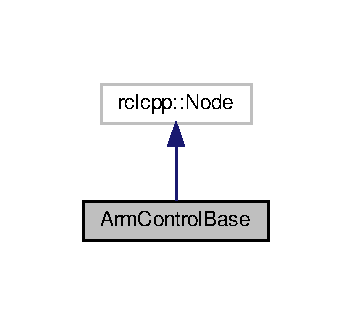
\includegraphics[width=169pt]{classArmControlBase__inherit__graph}
\end{center}
\end{figure}


Collaboration diagram for Arm\+Control\+Base\+:
\nopagebreak
\begin{figure}[H]
\begin{center}
\leavevmode
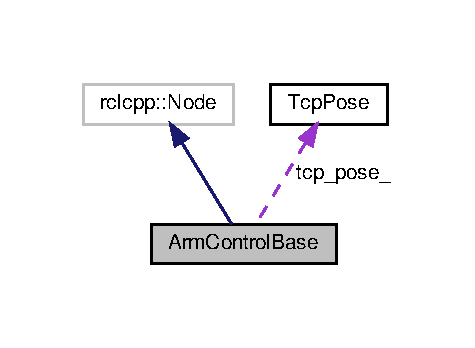
\includegraphics[width=228pt]{classArmControlBase__coll__graph}
\end{center}
\end{figure}
\subsection*{Public Member Functions}
\begin{DoxyCompactItemize}
\item 
\hyperlink{classArmControlBase_a5e5d5e6aaf2cf2957266353630f528fa}{Arm\+Control\+Base} (const std\+::string node\+\_\+name, const rclcpp\+::\+Node\+Options \&options)
\begin{DoxyCompactList}\small\item\em Constructor of class \hyperlink{classArmControlBase}{Arm\+Control\+Base}. \end{DoxyCompactList}\item 
\mbox{\Hypertarget{classArmControlBase_aa9bd5efabe0650f102dd42ee88adc820}\label{classArmControlBase_aa9bd5efabe0650f102dd42ee88adc820}} 
virtual \hyperlink{classArmControlBase_aa9bd5efabe0650f102dd42ee88adc820}{$\sim$\+Arm\+Control\+Base} ()
\begin{DoxyCompactList}\small\item\em Default destructor of class \hyperlink{classArmControlBase}{Arm\+Control\+Base}. \end{DoxyCompactList}\item 
virtual bool \hyperlink{classArmControlBase_aafd6f3d4bb78472087f53bfab89f9cb1}{move\+To\+Tcp\+Pose} (double x, double y, double z, double alpha, double beta, double gamma, double vel, double acc)=0
\begin{DoxyCompactList}\small\item\em Move the robot end-\/effector to a goal pose (position and orientation) w.\+r.\+t the robot base in 3D Cartesian space. \end{DoxyCompactList}\item 
virtual bool \hyperlink{classArmControlBase_a54c69305477aac08b8389d11920ccf5d}{move\+To\+Tcp\+Pose} (const Eigen\+::\+Isometry3d \&pose, double vel, double acc)
\begin{DoxyCompactList}\small\item\em Move the robot end-\/effector to a goal pose (position and orientation) w.\+r.\+t the robot base in 3D Cartesian space. \end{DoxyCompactList}\item 
virtual bool \hyperlink{classArmControlBase_a66a2e439066819b120405b2c0cbeaac5}{move\+To\+Tcp\+Pose} (const geometry\+\_\+msgs\+::msg\+::\+Pose\+Stamped \&pose\+\_\+stamped, double vel, double acc)
\begin{DoxyCompactList}\small\item\em Move the robot end-\/effector to a goal pose (position and orientation) w.\+r.\+t the robot base in 3D Cartesian space. \end{DoxyCompactList}\item 
virtual bool \hyperlink{classArmControlBase_aa78d160ed71fff8b9669536c953acf24}{move\+To\+Joint\+Values} (const std\+::vector$<$ double $>$ \&joint\+\_\+values, double vel, double acc)=0
\begin{DoxyCompactList}\small\item\em Move the robot to a joint value goal. \end{DoxyCompactList}\item 
virtual bool \hyperlink{classArmControlBase_aa2aeceddba7e0bfe1166199633dd3cba}{open} (const double distance=0)=0
\begin{DoxyCompactList}\small\item\em Open the robot gripper and make it ready for grasping. \end{DoxyCompactList}\item 
virtual bool \hyperlink{classArmControlBase_a7d767299ad4e2e087a89d911b93467c0}{close} (const double distance=0)=0
\begin{DoxyCompactList}\small\item\em Close the robot gripper and let it grasp an object. \end{DoxyCompactList}\item 
virtual bool \hyperlink{classArmControlBase_a447f53d50fb181492bf66a26e05c9aea}{pick} (double x, double y, double z, double alpha, double beta, double gamma, double vel, double acc, double vel\+\_\+scale, double approach)
\begin{DoxyCompactList}\small\item\em Make the robot arm to pick an object from a grasp pose w.\+r.\+t the robot base. \end{DoxyCompactList}\item 
virtual bool \hyperlink{classArmControlBase_aee6005df5aab9aa52d42b3adaf370856}{pick} (const geometry\+\_\+msgs\+::msg\+::\+Pose\+Stamped \&pose\+\_\+stamped, double vel, double acc, double vel\+\_\+scale, double approach)
\begin{DoxyCompactList}\small\item\em Make the robot arm to pick an object from a grasp pose w.\+r.\+t the robot base. \end{DoxyCompactList}\item 
virtual bool \hyperlink{classArmControlBase_a7bf0dfe8e090e9e334b6c3fcc47e8583}{place} (double x, double y, double z, double alpha, double beta, double gamma, double vel, double acc, double vel\+\_\+scale, double retract)
\begin{DoxyCompactList}\small\item\em Make the robot arm to place an object from a place pose w.\+r.\+t the robot base. \end{DoxyCompactList}\item 
virtual bool \hyperlink{classArmControlBase_a3bb794da7b45bce3e2e16b3cecb21379}{place} (const geometry\+\_\+msgs\+::msg\+::\+Pose\+Stamped \&pose\+\_\+stamped, double vel, double acc, double vel\+\_\+scale, double retract)
\begin{DoxyCompactList}\small\item\em Make the robot arm to place an object from a place pose w.\+r.\+t the robot base. \end{DoxyCompactList}\item 
void \hyperlink{classArmControlBase_a5163e7091cd7d1a9a12121cfaefc6330}{to\+Tcp\+Pose} (const geometry\+\_\+msgs\+::msg\+::\+Pose\+Stamped \&pose\+\_\+stamped, \hyperlink{structTcpPose}{Tcp\+Pose} \&tcp\+\_\+pose)
\begin{DoxyCompactList}\small\item\em Convert {\bfseries geometry\+\_\+msgs\+::msg\+::\+Pose\+Stamped} to \hyperlink{structTcpPose}{Tcp\+Pose}. \end{DoxyCompactList}\item 
void \hyperlink{classArmControlBase_a559aee5d6ea56cf5fba7e61c13b3ba8f}{to\+Tcp\+Pose} (const Eigen\+::\+Isometry3d \&pose, \hyperlink{structTcpPose}{Tcp\+Pose} \&tcp\+\_\+pose)
\begin{DoxyCompactList}\small\item\em Convert {\bfseries Eigen\+::\+Isometry3d} to \hyperlink{structTcpPose}{Tcp\+Pose}. \end{DoxyCompactList}\item 
virtual bool \hyperlink{classArmControlBase_a377f3ff5a7510e24c750db4878780dc4}{check\+Tcp\+Goal\+Arrived} (Eigen\+::\+Isometry3d \&tcp\+\_\+goal)
\begin{DoxyCompactList}\small\item\em Function to check if the end-\/effector arrived the goal pose. \end{DoxyCompactList}\item 
virtual bool \hyperlink{classArmControlBase_a3e695dc1f5d026fd81860f7d9d01c53b}{check\+Joint\+Value\+Goal\+Arrived} (const std\+::vector$<$ double $>$ \&joint\+\_\+goal)
\begin{DoxyCompactList}\small\item\em Function to check if the robot arm arrived the joint value goal. \end{DoxyCompactList}\item 
virtual void \hyperlink{classArmControlBase_ad7127c4d537e4cf386e0b315c4ae7386}{parse\+Args} ()=0
\begin{DoxyCompactList}\small\item\em Parse arguments. \end{DoxyCompactList}\item 
virtual bool \hyperlink{classArmControlBase_adcee7690990e054f03b146f769d77859}{start\+Loop} ()=0
\begin{DoxyCompactList}\small\item\em Start control loop. \end{DoxyCompactList}\item 
\mbox{\Hypertarget{classArmControlBase_a0e24e2e79df13e918e1ef317c4ac2ec1}\label{classArmControlBase_a0e24e2e79df13e918e1ef317c4ac2ec1}} 
virtual void \hyperlink{classArmControlBase_a0e24e2e79df13e918e1ef317c4ac2ec1}{publish\+T\+F\+Goal} ()
\begin{DoxyCompactList}\small\item\em Publish {\bfseries tf\+\_\+msg\+\_\+}. \end{DoxyCompactList}\item 
void \hyperlink{classArmControlBase_a81f9e2c00abd1eb665e3cca3e11972ab}{update\+T\+F\+Goal} (const geometry\+\_\+msgs\+::msg\+::\+Pose\+Stamped \&pose\+\_\+stamped)
\begin{DoxyCompactList}\small\item\em Update {\bfseries tf\+\_\+msg\+\_\+}. \end{DoxyCompactList}\item 
Eigen\+::\+Vector3d \hyperlink{classArmControlBase_aca29358591477ee195f01748266d7e9b}{get\+Unit\+Approach\+Vector} (const double \&alpha, const double \&beta, const double \&gamma)
\begin{DoxyCompactList}\small\item\em This function is used to rotate a unit vector along z axis, i.\+e. (0, 0, 1) by the assigned rpy euler angles. \end{DoxyCompactList}\end{DoxyCompactItemize}
\subsection*{Protected Attributes}
\begin{DoxyCompactItemize}
\item 
\mbox{\Hypertarget{classArmControlBase_ad73e15cce746d086b3f526d814362337}\label{classArmControlBase_ad73e15cce746d086b3f526d814362337}} 
rclcpp\+::\+Publisher$<$ sensor\+\_\+msgs\+::msg\+::\+Joint\+State $>$\+::Shared\+Ptr \hyperlink{classArmControlBase_ad73e15cce746d086b3f526d814362337}{joint\+\_\+pub\+\_\+}
\begin{DoxyCompactList}\small\item\em Joint state publisher. \end{DoxyCompactList}\item 
\mbox{\Hypertarget{classArmControlBase_ac8778720f435d3cdd44b7efb6dd76b3b}\label{classArmControlBase_ac8778720f435d3cdd44b7efb6dd76b3b}} 
std\+::vector$<$ std\+::string $>$ \hyperlink{classArmControlBase_ac8778720f435d3cdd44b7efb6dd76b3b}{joint\+\_\+names\+\_\+}
\begin{DoxyCompactList}\small\item\em Joint names. \end{DoxyCompactList}\item 
\mbox{\Hypertarget{classArmControlBase_a2d6a98c9218fc0056303a3a544e4fe37}\label{classArmControlBase_a2d6a98c9218fc0056303a3a544e4fe37}} 
\hyperlink{structTcpPose}{Tcp\+Pose} \hyperlink{classArmControlBase_a2d6a98c9218fc0056303a3a544e4fe37}{tcp\+\_\+pose\+\_\+}
\begin{DoxyCompactList}\small\item\em Current end-\/effctor pose. \end{DoxyCompactList}\item 
\mbox{\Hypertarget{classArmControlBase_a6262c793e6c778a9ad71037918d57f41}\label{classArmControlBase_a6262c793e6c778a9ad71037918d57f41}} 
std\+::vector$<$ double $>$ \hyperlink{classArmControlBase_a6262c793e6c778a9ad71037918d57f41}{joint\+\_\+values\+\_\+}
\begin{DoxyCompactList}\small\item\em Current joint value. \end{DoxyCompactList}\item 
\mbox{\Hypertarget{classArmControlBase_a1965ad8ee920b1ffc9d1bddbbf053edd}\label{classArmControlBase_a1965ad8ee920b1ffc9d1bddbbf053edd}} 
std\+::mutex \hyperlink{classArmControlBase_a1965ad8ee920b1ffc9d1bddbbf053edd}{m\+\_\+}
\begin{DoxyCompactList}\small\item\em Mutex to guard the tcp\+\_\+pose\+\_\+ usage. \end{DoxyCompactList}\item 
\mbox{\Hypertarget{classArmControlBase_ab21a9f771990d5b4c88a95040473ce39}\label{classArmControlBase_ab21a9f771990d5b4c88a95040473ce39}} 
double \hyperlink{classArmControlBase_ab21a9f771990d5b4c88a95040473ce39}{time\+\_\+out\+\_\+}
\begin{DoxyCompactList}\small\item\em Time duration to finish a pick or place task. \end{DoxyCompactList}\item 
\mbox{\Hypertarget{classArmControlBase_a31f7693c570cdb64b5c2534ca0a0413e}\label{classArmControlBase_a31f7693c570cdb64b5c2534ca0a0413e}} 
std\+::thread \hyperlink{classArmControlBase_a31f7693c570cdb64b5c2534ca0a0413e}{tf\+\_\+thread\+\_\+}
\begin{DoxyCompactList}\small\item\em Thread to publish tf pose. \end{DoxyCompactList}\item 
\mbox{\Hypertarget{classArmControlBase_af8ca0c0155b34197923554470172f858}\label{classArmControlBase_af8ca0c0155b34197923554470172f858}} 
geometry\+\_\+msgs\+::msg\+::\+Transform\+Stamped \hyperlink{classArmControlBase_af8ca0c0155b34197923554470172f858}{tf\+\_\+msg\+\_\+}
\begin{DoxyCompactList}\small\item\em TF message converted from the pose stamped input to the move or pick/place commands. \end{DoxyCompactList}\item 
\mbox{\Hypertarget{classArmControlBase_a1b16ae75e1410202c4add9b229f546c4}\label{classArmControlBase_a1b16ae75e1410202c4add9b229f546c4}} 
tf2\+\_\+ros\+::\+Static\+Transform\+Broadcaster \hyperlink{classArmControlBase_a1b16ae75e1410202c4add9b229f546c4}{broadcaster\+\_\+}
\begin{DoxyCompactList}\small\item\em TF broadcaster. \end{DoxyCompactList}\end{DoxyCompactItemize}


\subsection{Detailed Description}
Robot arm control interface. 

\subsection{Constructor \& Destructor Documentation}
\mbox{\Hypertarget{classArmControlBase_a5e5d5e6aaf2cf2957266353630f528fa}\label{classArmControlBase_a5e5d5e6aaf2cf2957266353630f528fa}} 
\index{Arm\+Control\+Base@{Arm\+Control\+Base}!Arm\+Control\+Base@{Arm\+Control\+Base}}
\index{Arm\+Control\+Base@{Arm\+Control\+Base}!Arm\+Control\+Base@{Arm\+Control\+Base}}
\subsubsection{\texorpdfstring{Arm\+Control\+Base()}{ArmControlBase()}}
{\footnotesize\ttfamily Arm\+Control\+Base\+::\+Arm\+Control\+Base (\begin{DoxyParamCaption}\item[{const std\+::string}]{node\+\_\+name,  }\item[{const rclcpp\+::\+Node\+Options \&}]{options }\end{DoxyParamCaption})\hspace{0.3cm}{\ttfamily [inline]}}



Constructor of class \hyperlink{classArmControlBase}{Arm\+Control\+Base}. 


\begin{DoxyParams}{Parameters}
{\em node\+\_\+name} & The name of the R\+O\+S2 node. \\
\hline
{\em options} & R\+O\+S2 node options. \\
\hline
\end{DoxyParams}


\subsection{Member Function Documentation}
\mbox{\Hypertarget{classArmControlBase_a3e695dc1f5d026fd81860f7d9d01c53b}\label{classArmControlBase_a3e695dc1f5d026fd81860f7d9d01c53b}} 
\index{Arm\+Control\+Base@{Arm\+Control\+Base}!check\+Joint\+Value\+Goal\+Arrived@{check\+Joint\+Value\+Goal\+Arrived}}
\index{check\+Joint\+Value\+Goal\+Arrived@{check\+Joint\+Value\+Goal\+Arrived}!Arm\+Control\+Base@{Arm\+Control\+Base}}
\subsubsection{\texorpdfstring{check\+Joint\+Value\+Goal\+Arrived()}{checkJointValueGoalArrived()}}
{\footnotesize\ttfamily bool Arm\+Control\+Base\+::check\+Joint\+Value\+Goal\+Arrived (\begin{DoxyParamCaption}\item[{const std\+::vector$<$ double $>$ \&}]{joint\+\_\+goal }\end{DoxyParamCaption})\hspace{0.3cm}{\ttfamily [virtual]}}



Function to check if the robot arm arrived the joint value goal. 


\begin{DoxyParams}{Parameters}
{\em joint\+\_\+values} & Joint value goal of the robot arm. \\
\hline
\end{DoxyParams}
\begin{DoxyReturn}{Returns}
If the robot arrived the joint value goal within a {\bfseries time\+\_\+out\+\_\+} duration, return true. Otherwise, return false. 
\end{DoxyReturn}
\mbox{\Hypertarget{classArmControlBase_a377f3ff5a7510e24c750db4878780dc4}\label{classArmControlBase_a377f3ff5a7510e24c750db4878780dc4}} 
\index{Arm\+Control\+Base@{Arm\+Control\+Base}!check\+Tcp\+Goal\+Arrived@{check\+Tcp\+Goal\+Arrived}}
\index{check\+Tcp\+Goal\+Arrived@{check\+Tcp\+Goal\+Arrived}!Arm\+Control\+Base@{Arm\+Control\+Base}}
\subsubsection{\texorpdfstring{check\+Tcp\+Goal\+Arrived()}{checkTcpGoalArrived()}}
{\footnotesize\ttfamily bool Arm\+Control\+Base\+::check\+Tcp\+Goal\+Arrived (\begin{DoxyParamCaption}\item[{Eigen\+::\+Isometry3d \&}]{tcp\+\_\+goal }\end{DoxyParamCaption})\hspace{0.3cm}{\ttfamily [virtual]}}



Function to check if the end-\/effector arrived the goal pose. 


\begin{DoxyParams}{Parameters}
{\em tcp\+\_\+goal} & Goal pose of the end-\/effector. \\
\hline
\end{DoxyParams}
\begin{DoxyReturn}{Returns}
If the end-\/effector arrived the goal pose within a {\bfseries time\+\_\+out\+\_\+} duration, return true. Otherwise, return false. 
\end{DoxyReturn}
\mbox{\Hypertarget{classArmControlBase_a7d767299ad4e2e087a89d911b93467c0}\label{classArmControlBase_a7d767299ad4e2e087a89d911b93467c0}} 
\index{Arm\+Control\+Base@{Arm\+Control\+Base}!close@{close}}
\index{close@{close}!Arm\+Control\+Base@{Arm\+Control\+Base}}
\subsubsection{\texorpdfstring{close()}{close()}}
{\footnotesize\ttfamily virtual bool Arm\+Control\+Base\+::close (\begin{DoxyParamCaption}\item[{const double}]{distance = {\ttfamily 0} }\end{DoxyParamCaption})\hspace{0.3cm}{\ttfamily [pure virtual]}}



Close the robot gripper and let it grasp an object. 


\begin{DoxyParams}{Parameters}
{\em distance} & How large the fingers of the gripper close. \\
\hline
\end{DoxyParams}
\begin{DoxyReturn}{Returns}
If the robot successfully receives the \char`\"{}close\char`\"{} command, return true. Otherwise, return false. 
\end{DoxyReturn}
\mbox{\Hypertarget{classArmControlBase_aca29358591477ee195f01748266d7e9b}\label{classArmControlBase_aca29358591477ee195f01748266d7e9b}} 
\index{Arm\+Control\+Base@{Arm\+Control\+Base}!get\+Unit\+Approach\+Vector@{get\+Unit\+Approach\+Vector}}
\index{get\+Unit\+Approach\+Vector@{get\+Unit\+Approach\+Vector}!Arm\+Control\+Base@{Arm\+Control\+Base}}
\subsubsection{\texorpdfstring{get\+Unit\+Approach\+Vector()}{getUnitApproachVector()}}
{\footnotesize\ttfamily Eigen\+::\+Vector3d Arm\+Control\+Base\+::get\+Unit\+Approach\+Vector (\begin{DoxyParamCaption}\item[{const double \&}]{alpha,  }\item[{const double \&}]{beta,  }\item[{const double \&}]{gamma }\end{DoxyParamCaption})}



This function is used to rotate a unit vector along z axis, i.\+e. (0, 0, 1) by the assigned rpy euler angles. 


\begin{DoxyParams}{Parameters}
{\em alpha} & Rotation euler angle around X axis. \\
\hline
{\em beta} & Rotation euler angle around Y axis. \\
\hline
{\em gamma} & Rotation euler angle around Z axis. \\
\hline
\end{DoxyParams}
\mbox{\Hypertarget{classArmControlBase_aa78d160ed71fff8b9669536c953acf24}\label{classArmControlBase_aa78d160ed71fff8b9669536c953acf24}} 
\index{Arm\+Control\+Base@{Arm\+Control\+Base}!move\+To\+Joint\+Values@{move\+To\+Joint\+Values}}
\index{move\+To\+Joint\+Values@{move\+To\+Joint\+Values}!Arm\+Control\+Base@{Arm\+Control\+Base}}
\subsubsection{\texorpdfstring{move\+To\+Joint\+Values()}{moveToJointValues()}}
{\footnotesize\ttfamily virtual bool Arm\+Control\+Base\+::move\+To\+Joint\+Values (\begin{DoxyParamCaption}\item[{const std\+::vector$<$ double $>$ \&}]{joint\+\_\+values,  }\item[{double}]{vel,  }\item[{double}]{acc }\end{DoxyParamCaption})\hspace{0.3cm}{\ttfamily [pure virtual]}}



Move the robot to a joint value goal. 


\begin{DoxyParams}{Parameters}
{\em joint\+\_\+values} & Goal joint values, the number of joints depends on the robot arm model. \\
\hline
{\em vel} & Max joint velocity. \\
\hline
{\em acc} & Max joint acceleration. \\
\hline
\end{DoxyParams}
\begin{DoxyReturn}{Returns}
If the robot successfully receives the \char`\"{}move\char`\"{} command, return True. Otherwise, return false. 
\end{DoxyReturn}
\mbox{\Hypertarget{classArmControlBase_aafd6f3d4bb78472087f53bfab89f9cb1}\label{classArmControlBase_aafd6f3d4bb78472087f53bfab89f9cb1}} 
\index{Arm\+Control\+Base@{Arm\+Control\+Base}!move\+To\+Tcp\+Pose@{move\+To\+Tcp\+Pose}}
\index{move\+To\+Tcp\+Pose@{move\+To\+Tcp\+Pose}!Arm\+Control\+Base@{Arm\+Control\+Base}}
\subsubsection{\texorpdfstring{move\+To\+Tcp\+Pose()}{moveToTcpPose()}\hspace{0.1cm}{\footnotesize\ttfamily [1/3]}}
{\footnotesize\ttfamily virtual bool Arm\+Control\+Base\+::move\+To\+Tcp\+Pose (\begin{DoxyParamCaption}\item[{double}]{x,  }\item[{double}]{y,  }\item[{double}]{z,  }\item[{double}]{alpha,  }\item[{double}]{beta,  }\item[{double}]{gamma,  }\item[{double}]{vel,  }\item[{double}]{acc }\end{DoxyParamCaption})\hspace{0.3cm}{\ttfamily [pure virtual]}}



Move the robot end-\/effector to a goal pose (position and orientation) w.\+r.\+t the robot base in 3D Cartesian space. 


\begin{DoxyParams}{Parameters}
{\em x} & Goal position on X dimension. \\
\hline
{\em y} & Goal position on Y dimension. \\
\hline
{\em z} & Goal position on Z dimension. \\
\hline
{\em alpha} & Goal rotation euler angle along X axis. \\
\hline
{\em beta} & Goal rotation euler angle along Y axis. \\
\hline
{\em gamma} & Goal rotation euler angle along Z axis. \\
\hline
{\em vel} & Max joint velocity. \\
\hline
{\em acc} & Max joint acceleration. \\
\hline
\end{DoxyParams}
\begin{DoxyReturn}{Returns}
If the robot successfully receives the \char`\"{}move\char`\"{} command, return True. Otherwise, return false. 
\end{DoxyReturn}
\mbox{\Hypertarget{classArmControlBase_a54c69305477aac08b8389d11920ccf5d}\label{classArmControlBase_a54c69305477aac08b8389d11920ccf5d}} 
\index{Arm\+Control\+Base@{Arm\+Control\+Base}!move\+To\+Tcp\+Pose@{move\+To\+Tcp\+Pose}}
\index{move\+To\+Tcp\+Pose@{move\+To\+Tcp\+Pose}!Arm\+Control\+Base@{Arm\+Control\+Base}}
\subsubsection{\texorpdfstring{move\+To\+Tcp\+Pose()}{moveToTcpPose()}\hspace{0.1cm}{\footnotesize\ttfamily [2/3]}}
{\footnotesize\ttfamily bool Arm\+Control\+Base\+::move\+To\+Tcp\+Pose (\begin{DoxyParamCaption}\item[{const Eigen\+::\+Isometry3d \&}]{pose,  }\item[{double}]{vel,  }\item[{double}]{acc }\end{DoxyParamCaption})\hspace{0.3cm}{\ttfamily [virtual]}}



Move the robot end-\/effector to a goal pose (position and orientation) w.\+r.\+t the robot base in 3D Cartesian space. 


\begin{DoxyParams}{Parameters}
{\em pose} & Goal pose as a Eigen transform (Isometry3d). \\
\hline
{\em vel} & Max joint velocity. \\
\hline
{\em acc} & Max joint acceleration. \\
\hline
\end{DoxyParams}
\begin{DoxyReturn}{Returns}
If the robot successfully receives the \char`\"{}move\char`\"{} command, return True. Otherwise, return false. 
\end{DoxyReturn}
\mbox{\Hypertarget{classArmControlBase_a66a2e439066819b120405b2c0cbeaac5}\label{classArmControlBase_a66a2e439066819b120405b2c0cbeaac5}} 
\index{Arm\+Control\+Base@{Arm\+Control\+Base}!move\+To\+Tcp\+Pose@{move\+To\+Tcp\+Pose}}
\index{move\+To\+Tcp\+Pose@{move\+To\+Tcp\+Pose}!Arm\+Control\+Base@{Arm\+Control\+Base}}
\subsubsection{\texorpdfstring{move\+To\+Tcp\+Pose()}{moveToTcpPose()}\hspace{0.1cm}{\footnotesize\ttfamily [3/3]}}
{\footnotesize\ttfamily bool Arm\+Control\+Base\+::move\+To\+Tcp\+Pose (\begin{DoxyParamCaption}\item[{const geometry\+\_\+msgs\+::msg\+::\+Pose\+Stamped \&}]{pose\+\_\+stamped,  }\item[{double}]{vel,  }\item[{double}]{acc }\end{DoxyParamCaption})\hspace{0.3cm}{\ttfamily [virtual]}}



Move the robot end-\/effector to a goal pose (position and orientation) w.\+r.\+t the robot base in 3D Cartesian space. 


\begin{DoxyParams}{Parameters}
{\em pose\+\_\+stamped} & Goal pose as geometry\+\_\+msgs/\+Pose\+Stamped. \\
\hline
{\em vel} & Max joint velocity. \\
\hline
{\em acc} & Max joint acceleration. \\
\hline
\end{DoxyParams}
\begin{DoxyReturn}{Returns}
If the robot successfully receives the \char`\"{}move\char`\"{} command, return True. Otherwise, return false. 
\end{DoxyReturn}
\mbox{\Hypertarget{classArmControlBase_aa2aeceddba7e0bfe1166199633dd3cba}\label{classArmControlBase_aa2aeceddba7e0bfe1166199633dd3cba}} 
\index{Arm\+Control\+Base@{Arm\+Control\+Base}!open@{open}}
\index{open@{open}!Arm\+Control\+Base@{Arm\+Control\+Base}}
\subsubsection{\texorpdfstring{open()}{open()}}
{\footnotesize\ttfamily virtual bool Arm\+Control\+Base\+::open (\begin{DoxyParamCaption}\item[{const double}]{distance = {\ttfamily 0} }\end{DoxyParamCaption})\hspace{0.3cm}{\ttfamily [pure virtual]}}



Open the robot gripper and make it ready for grasping. 


\begin{DoxyParams}{Parameters}
{\em distance} & How large the fingers of the gripper open. \\
\hline
\end{DoxyParams}
\begin{DoxyReturn}{Returns}
If the robot successfully receives the \char`\"{}open\char`\"{} command, return true. Otherwise, return false. 
\end{DoxyReturn}
\mbox{\Hypertarget{classArmControlBase_ad7127c4d537e4cf386e0b315c4ae7386}\label{classArmControlBase_ad7127c4d537e4cf386e0b315c4ae7386}} 
\index{Arm\+Control\+Base@{Arm\+Control\+Base}!parse\+Args@{parse\+Args}}
\index{parse\+Args@{parse\+Args}!Arm\+Control\+Base@{Arm\+Control\+Base}}
\subsubsection{\texorpdfstring{parse\+Args()}{parseArgs()}}
{\footnotesize\ttfamily virtual void Arm\+Control\+Base\+::parse\+Args (\begin{DoxyParamCaption}{ }\end{DoxyParamCaption})\hspace{0.3cm}{\ttfamily [pure virtual]}}



Parse arguments. 

This function is used to parse the communication or control configuration parameters. A common method is defining the configuration parameters in a .yaml file, then loading them as R\+O\+S2 node parameters and parsing them by R\+O\+S2 node parameter client. \mbox{\Hypertarget{classArmControlBase_a447f53d50fb181492bf66a26e05c9aea}\label{classArmControlBase_a447f53d50fb181492bf66a26e05c9aea}} 
\index{Arm\+Control\+Base@{Arm\+Control\+Base}!pick@{pick}}
\index{pick@{pick}!Arm\+Control\+Base@{Arm\+Control\+Base}}
\subsubsection{\texorpdfstring{pick()}{pick()}\hspace{0.1cm}{\footnotesize\ttfamily [1/2]}}
{\footnotesize\ttfamily bool Arm\+Control\+Base\+::pick (\begin{DoxyParamCaption}\item[{double}]{x,  }\item[{double}]{y,  }\item[{double}]{z,  }\item[{double}]{alpha,  }\item[{double}]{beta,  }\item[{double}]{gamma,  }\item[{double}]{vel,  }\item[{double}]{acc,  }\item[{double}]{vel\+\_\+scale,  }\item[{double}]{approach }\end{DoxyParamCaption})\hspace{0.3cm}{\ttfamily [virtual]}}



Make the robot arm to pick an object from a grasp pose w.\+r.\+t the robot base. 

This function defines a sequence of motions\+:
\begin{DoxyEnumerate}
\item Move the end-\/effector to a pose above the object.
\item Open gripper.
\item Stretch the end-\/effector along its Z axis to the grasp pose that gripper can grasp the object.
\item Close gripper.
\item Move the end-\/effector back to the pose above the object.
\end{DoxyEnumerate}


\begin{DoxyParams}{Parameters}
{\em x} & Position of grasp pose on X dimension. \\
\hline
{\em y} & Position of grasp pose on Y dimension. \\
\hline
{\em z} & Position of grasp pose on Z dimension. \\
\hline
{\em alpha} & Rotation euler angle of grasp pose along X axis. \\
\hline
{\em beta} & Rotation euler angle of grasp pose along Y axis. \\
\hline
{\em gamma} & Rotation euler angle of grasp pose along Z axis. \\
\hline
{\em vel} & Max joint velocity. \\
\hline
{\em acc} & Max joint acceleration. \\
\hline
{\em vel\+\_\+scale} & Scale factor to slow down the end-\/effector velocity, when it stretch to or move back from the grasp pose. \\
\hline
{\em approach} & The stretch distance. \\
\hline
\end{DoxyParams}
\begin{DoxyReturn}{Returns}
If the robot successfully finishes the \char`\"{}pick\char`\"{} motions, return True. Otherwise, return false. 
\end{DoxyReturn}
\begin{DoxyNote}{Note}
The grasp pose should have Z axis point out from the end-\/effector link. 
\end{DoxyNote}
\mbox{\Hypertarget{classArmControlBase_aee6005df5aab9aa52d42b3adaf370856}\label{classArmControlBase_aee6005df5aab9aa52d42b3adaf370856}} 
\index{Arm\+Control\+Base@{Arm\+Control\+Base}!pick@{pick}}
\index{pick@{pick}!Arm\+Control\+Base@{Arm\+Control\+Base}}
\subsubsection{\texorpdfstring{pick()}{pick()}\hspace{0.1cm}{\footnotesize\ttfamily [2/2]}}
{\footnotesize\ttfamily bool Arm\+Control\+Base\+::pick (\begin{DoxyParamCaption}\item[{const geometry\+\_\+msgs\+::msg\+::\+Pose\+Stamped \&}]{pose\+\_\+stamped,  }\item[{double}]{vel,  }\item[{double}]{acc,  }\item[{double}]{vel\+\_\+scale,  }\item[{double}]{approach }\end{DoxyParamCaption})\hspace{0.3cm}{\ttfamily [virtual]}}



Make the robot arm to pick an object from a grasp pose w.\+r.\+t the robot base. 

This function defines a sequence of motions\+:
\begin{DoxyEnumerate}
\item Move the end-\/effector to a pose above the object.
\item Open gripper.
\item Stretch the end-\/effector along its Z axis to the grasp pose that gripper can grasp the object.
\item Close gripper.
\item Move the end-\/effector back to the pose above the object.
\end{DoxyEnumerate}


\begin{DoxyParams}{Parameters}
{\em pose\+\_\+stamped} & Pose received from the grasp planning algorithm. See also \href{https://github.com/intel/ros2_grasp_library}{\tt https\+://github.\+com/intel/ros2\+\_\+grasp\+\_\+library}. \\
\hline
{\em vel} & Max joint velocity. \\
\hline
{\em acc} & Max joint acceleration. \\
\hline
{\em vel\+\_\+scale} & Scale factor to slow down the end-\/effector velocity, when it stretch to or move back from the grasp pose. \\
\hline
{\em approach} & The stretch distance. \\
\hline
\end{DoxyParams}
\begin{DoxyReturn}{Returns}
If the robot successfully finishes the \char`\"{}pick\char`\"{} motions, return True. Otherwise, return false. 
\end{DoxyReturn}
\begin{DoxyNote}{Note}
The grasp pose should have Z axis point out from the end-\/effector link. 
\end{DoxyNote}
\mbox{\Hypertarget{classArmControlBase_a7bf0dfe8e090e9e334b6c3fcc47e8583}\label{classArmControlBase_a7bf0dfe8e090e9e334b6c3fcc47e8583}} 
\index{Arm\+Control\+Base@{Arm\+Control\+Base}!place@{place}}
\index{place@{place}!Arm\+Control\+Base@{Arm\+Control\+Base}}
\subsubsection{\texorpdfstring{place()}{place()}\hspace{0.1cm}{\footnotesize\ttfamily [1/2]}}
{\footnotesize\ttfamily bool Arm\+Control\+Base\+::place (\begin{DoxyParamCaption}\item[{double}]{x,  }\item[{double}]{y,  }\item[{double}]{z,  }\item[{double}]{alpha,  }\item[{double}]{beta,  }\item[{double}]{gamma,  }\item[{double}]{vel,  }\item[{double}]{acc,  }\item[{double}]{vel\+\_\+scale,  }\item[{double}]{retract }\end{DoxyParamCaption})\hspace{0.3cm}{\ttfamily [virtual]}}



Make the robot arm to place an object from a place pose w.\+r.\+t the robot base. 

This function defines a sequence of motions\+:
\begin{DoxyEnumerate}
\item Move the end-\/effector to a pre-\/place pose.
\item Stretch the end-\/effector along its Z axis to the place pose.
\item Open gripper.
\item Move the end-\/effector back to the pre-\/place pose.
\end{DoxyEnumerate}


\begin{DoxyParams}{Parameters}
{\em x} & Position of place pose on X dimension. \\
\hline
{\em y} & Position of place pose on Y dimension. \\
\hline
{\em z} & Position of place pose on Z dimension. \\
\hline
{\em alpha} & Rotation euler angle of place pose along X axis. \\
\hline
{\em beta} & Rotation euler angle of place pose along Y axis. \\
\hline
{\em gamma} & Rotation euler angle of place pose along Z axis. \\
\hline
{\em vel} & Max joint velocity. \\
\hline
{\em acc} & Max joint acceleration. \\
\hline
{\em vel\+\_\+scale} & Scale factor to slow down the end-\/effector velocity, when it stretch to or move back from the place pose. \\
\hline
{\em retract} & The retract distance from the place pose. \\
\hline
\end{DoxyParams}
\begin{DoxyReturn}{Returns}
If the robot successfully finishes the \char`\"{}place\char`\"{} motions, return True. Otherwise, return false. 
\end{DoxyReturn}
\begin{DoxyNote}{Note}
The place pose should have Z axis point out from the end-\/effector link. 
\end{DoxyNote}
\mbox{\Hypertarget{classArmControlBase_a3bb794da7b45bce3e2e16b3cecb21379}\label{classArmControlBase_a3bb794da7b45bce3e2e16b3cecb21379}} 
\index{Arm\+Control\+Base@{Arm\+Control\+Base}!place@{place}}
\index{place@{place}!Arm\+Control\+Base@{Arm\+Control\+Base}}
\subsubsection{\texorpdfstring{place()}{place()}\hspace{0.1cm}{\footnotesize\ttfamily [2/2]}}
{\footnotesize\ttfamily bool Arm\+Control\+Base\+::place (\begin{DoxyParamCaption}\item[{const geometry\+\_\+msgs\+::msg\+::\+Pose\+Stamped \&}]{pose\+\_\+stamped,  }\item[{double}]{vel,  }\item[{double}]{acc,  }\item[{double}]{vel\+\_\+scale,  }\item[{double}]{retract }\end{DoxyParamCaption})\hspace{0.3cm}{\ttfamily [virtual]}}



Make the robot arm to place an object from a place pose w.\+r.\+t the robot base. 

This function defines a sequence of motions\+:
\begin{DoxyEnumerate}
\item Move the end-\/effector to a pre-\/place pose.
\item Stretch the end-\/effector along its Z axis to the place pose.
\item Open gripper.
\item Move the end-\/effector back to the pre-\/place pose.
\end{DoxyEnumerate}


\begin{DoxyParams}{Parameters}
{\em pose\+\_\+stamped} & Pose of the end-\/effector to place an object. \\
\hline
{\em vel} & Max joint velocity. \\
\hline
{\em acc} & Max joint acceleration. \\
\hline
{\em vel\+\_\+scale} & Scale factor to slow down the end-\/effector velocity, when it stretch to or retract back from the place pose. \\
\hline
{\em retract} & The retract distance from the place pose. \\
\hline
\end{DoxyParams}
\begin{DoxyReturn}{Returns}
If the robot successfully finishes the \char`\"{}place\char`\"{} motions, return True. Otherwise, return false. 
\end{DoxyReturn}
\begin{DoxyNote}{Note}
The place pose should have Z axis point out from the end-\/effector link. 
\end{DoxyNote}
\mbox{\Hypertarget{classArmControlBase_adcee7690990e054f03b146f769d77859}\label{classArmControlBase_adcee7690990e054f03b146f769d77859}} 
\index{Arm\+Control\+Base@{Arm\+Control\+Base}!start\+Loop@{start\+Loop}}
\index{start\+Loop@{start\+Loop}!Arm\+Control\+Base@{Arm\+Control\+Base}}
\subsubsection{\texorpdfstring{start\+Loop()}{startLoop()}}
{\footnotesize\ttfamily virtual bool Arm\+Control\+Base\+::start\+Loop (\begin{DoxyParamCaption}{ }\end{DoxyParamCaption})\hspace{0.3cm}{\ttfamily [pure virtual]}}



Start control loop. 

This function is used to initialize the communication process and start the thread that reads and publishes the robot state. \mbox{\Hypertarget{classArmControlBase_a5163e7091cd7d1a9a12121cfaefc6330}\label{classArmControlBase_a5163e7091cd7d1a9a12121cfaefc6330}} 
\index{Arm\+Control\+Base@{Arm\+Control\+Base}!to\+Tcp\+Pose@{to\+Tcp\+Pose}}
\index{to\+Tcp\+Pose@{to\+Tcp\+Pose}!Arm\+Control\+Base@{Arm\+Control\+Base}}
\subsubsection{\texorpdfstring{to\+Tcp\+Pose()}{toTcpPose()}\hspace{0.1cm}{\footnotesize\ttfamily [1/2]}}
{\footnotesize\ttfamily void Arm\+Control\+Base\+::to\+Tcp\+Pose (\begin{DoxyParamCaption}\item[{const geometry\+\_\+msgs\+::msg\+::\+Pose\+Stamped \&}]{pose\+\_\+stamped,  }\item[{\hyperlink{structTcpPose}{Tcp\+Pose} \&}]{tcp\+\_\+pose }\end{DoxyParamCaption})}



Convert {\bfseries geometry\+\_\+msgs\+::msg\+::\+Pose\+Stamped} to \hyperlink{structTcpPose}{Tcp\+Pose}. 


\begin{DoxyParams}{Parameters}
{\em pose\+\_\+stamped} & Pose of the end-\/effector. \\
\hline
{\em tcp\+\_\+pose} & Variable to store the converted result. \\
\hline
\end{DoxyParams}
\mbox{\Hypertarget{classArmControlBase_a559aee5d6ea56cf5fba7e61c13b3ba8f}\label{classArmControlBase_a559aee5d6ea56cf5fba7e61c13b3ba8f}} 
\index{Arm\+Control\+Base@{Arm\+Control\+Base}!to\+Tcp\+Pose@{to\+Tcp\+Pose}}
\index{to\+Tcp\+Pose@{to\+Tcp\+Pose}!Arm\+Control\+Base@{Arm\+Control\+Base}}
\subsubsection{\texorpdfstring{to\+Tcp\+Pose()}{toTcpPose()}\hspace{0.1cm}{\footnotesize\ttfamily [2/2]}}
{\footnotesize\ttfamily void Arm\+Control\+Base\+::to\+Tcp\+Pose (\begin{DoxyParamCaption}\item[{const Eigen\+::\+Isometry3d \&}]{pose,  }\item[{\hyperlink{structTcpPose}{Tcp\+Pose} \&}]{tcp\+\_\+pose }\end{DoxyParamCaption})}



Convert {\bfseries Eigen\+::\+Isometry3d} to \hyperlink{structTcpPose}{Tcp\+Pose}. 


\begin{DoxyParams}{Parameters}
{\em pose} & Pose of the end-\/effector. \\
\hline
{\em tcp\+\_\+pose} & Variable to store the converted result. \\
\hline
\end{DoxyParams}
\mbox{\Hypertarget{classArmControlBase_a81f9e2c00abd1eb665e3cca3e11972ab}\label{classArmControlBase_a81f9e2c00abd1eb665e3cca3e11972ab}} 
\index{Arm\+Control\+Base@{Arm\+Control\+Base}!update\+T\+F\+Goal@{update\+T\+F\+Goal}}
\index{update\+T\+F\+Goal@{update\+T\+F\+Goal}!Arm\+Control\+Base@{Arm\+Control\+Base}}
\subsubsection{\texorpdfstring{update\+T\+F\+Goal()}{updateTFGoal()}}
{\footnotesize\ttfamily void Arm\+Control\+Base\+::update\+T\+F\+Goal (\begin{DoxyParamCaption}\item[{const geometry\+\_\+msgs\+::msg\+::\+Pose\+Stamped \&}]{pose\+\_\+stamped }\end{DoxyParamCaption})}



Update {\bfseries tf\+\_\+msg\+\_\+}. 


\begin{DoxyParams}{Parameters}
{\em pose\+\_\+stamped} & Pose goal input to the move or pick/place commands. \\
\hline
\end{DoxyParams}


The documentation for this class was generated from the following files\+:\begin{DoxyCompactItemize}
\item 
include/robot\+\_\+interface/\hyperlink{control__base_8hpp}{control\+\_\+base.\+hpp}\item 
src/\hyperlink{control__base_8cpp}{control\+\_\+base.\+cpp}\end{DoxyCompactItemize}

\hypertarget{structTcpPose}{}\section{Tcp\+Pose Struct Reference}
\label{structTcpPose}\index{Tcp\+Pose@{Tcp\+Pose}}


Data type to represent robot arm\textquotesingle{}s end-\/effector pose in 3D cartesian space.  




{\ttfamily \#include $<$control\+\_\+base.\+hpp$>$}

\subsection*{Public Attributes}
\begin{DoxyCompactItemize}
\item 
double \hyperlink{structTcpPose_ae394f2f7f9f51d60e868075712f87244}{x}
\item 
double \hyperlink{structTcpPose_a1050d339d788176b4323367a0150ad71}{y}
\item 
double \hyperlink{structTcpPose_a2c538c7a01a6950bcd9d6c2377f85ade}{z}
\item 
double \hyperlink{structTcpPose_ad9f0b5e0db1a7d559289180b1a046f63}{alpha}
\item 
double \hyperlink{structTcpPose_af07e5cf32da9710974e8b1eb3a654928}{beta}
\item 
double \hyperlink{structTcpPose_ae8efa3b9d6a4dfd78db315ffa28a23cc}{gamma}
\end{DoxyCompactItemize}


\subsection{Detailed Description}
Data type to represent robot arm\textquotesingle{}s end-\/effector pose in 3D cartesian space. 

\begin{DoxyNote}{Note}
{\bfseries T\+CP} stands for Tool Center Point. Usually it refers to The location on the end effector or tool of a robot manipulator whose position and orientation define the coordinates of the controlled object. 
\end{DoxyNote}


\subsection{Member Data Documentation}
\mbox{\Hypertarget{structTcpPose_ad9f0b5e0db1a7d559289180b1a046f63}\label{structTcpPose_ad9f0b5e0db1a7d559289180b1a046f63}} 
\index{Tcp\+Pose@{Tcp\+Pose}!alpha@{alpha}}
\index{alpha@{alpha}!Tcp\+Pose@{Tcp\+Pose}}
\subsubsection{\texorpdfstring{alpha}{alpha}}
{\footnotesize\ttfamily double Tcp\+Pose\+::alpha}

Euler angle of the rotation along X axis. \mbox{\Hypertarget{structTcpPose_af07e5cf32da9710974e8b1eb3a654928}\label{structTcpPose_af07e5cf32da9710974e8b1eb3a654928}} 
\index{Tcp\+Pose@{Tcp\+Pose}!beta@{beta}}
\index{beta@{beta}!Tcp\+Pose@{Tcp\+Pose}}
\subsubsection{\texorpdfstring{beta}{beta}}
{\footnotesize\ttfamily double Tcp\+Pose\+::beta}

Euler angle of the rotation along Y axis. \mbox{\Hypertarget{structTcpPose_ae8efa3b9d6a4dfd78db315ffa28a23cc}\label{structTcpPose_ae8efa3b9d6a4dfd78db315ffa28a23cc}} 
\index{Tcp\+Pose@{Tcp\+Pose}!gamma@{gamma}}
\index{gamma@{gamma}!Tcp\+Pose@{Tcp\+Pose}}
\subsubsection{\texorpdfstring{gamma}{gamma}}
{\footnotesize\ttfamily double Tcp\+Pose\+::gamma}

Euler angle of the rotation along Z axis. \mbox{\Hypertarget{structTcpPose_ae394f2f7f9f51d60e868075712f87244}\label{structTcpPose_ae394f2f7f9f51d60e868075712f87244}} 
\index{Tcp\+Pose@{Tcp\+Pose}!x@{x}}
\index{x@{x}!Tcp\+Pose@{Tcp\+Pose}}
\subsubsection{\texorpdfstring{x}{x}}
{\footnotesize\ttfamily double Tcp\+Pose\+::x}

Translation along X axis. \mbox{\Hypertarget{structTcpPose_a1050d339d788176b4323367a0150ad71}\label{structTcpPose_a1050d339d788176b4323367a0150ad71}} 
\index{Tcp\+Pose@{Tcp\+Pose}!y@{y}}
\index{y@{y}!Tcp\+Pose@{Tcp\+Pose}}
\subsubsection{\texorpdfstring{y}{y}}
{\footnotesize\ttfamily double Tcp\+Pose\+::y}

Translation along Y axis. \mbox{\Hypertarget{structTcpPose_a2c538c7a01a6950bcd9d6c2377f85ade}\label{structTcpPose_a2c538c7a01a6950bcd9d6c2377f85ade}} 
\index{Tcp\+Pose@{Tcp\+Pose}!z@{z}}
\index{z@{z}!Tcp\+Pose@{Tcp\+Pose}}
\subsubsection{\texorpdfstring{z}{z}}
{\footnotesize\ttfamily double Tcp\+Pose\+::z}

Translation along Z axis. 

The documentation for this struct was generated from the following file\+:\begin{DoxyCompactItemize}
\item 
include/robot\+\_\+interface/\hyperlink{control__base_8hpp}{control\+\_\+base.\+hpp}\end{DoxyCompactItemize}

\chapter{File Documentation}
\hypertarget{control__base_8hpp}{}\section{include/robot\+\_\+interface/control\+\_\+base.hpp File Reference}
\label{control__base_8hpp}\index{include/robot\+\_\+interface/control\+\_\+base.\+hpp@{include/robot\+\_\+interface/control\+\_\+base.\+hpp}}


Native robot control interface for visual manipulation.  


{\ttfamily \#include $<$mutex$>$}\newline
{\ttfamily \#include $<$thread$>$}\newline
{\ttfamily \#include $<$Eigen/\+Geometry$>$}\newline
{\ttfamily \#include $<$rclcpp/rclcpp.\+hpp$>$}\newline
{\ttfamily \#include $<$tf2\+\_\+eigen/tf2\+\_\+eigen.\+h$>$}\newline
{\ttfamily \#include $<$sensor\+\_\+msgs/msg/joint\+\_\+state.\+hpp$>$}\newline
{\ttfamily \#include $<$geometry\+\_\+msgs/msg/pose\+\_\+stamped.\+hpp$>$}\newline
{\ttfamily \#include $<$tf2\+\_\+ros/static\+\_\+transform\+\_\+broadcaster.\+h$>$}\newline
Include dependency graph for control\+\_\+base.\+hpp\+:
\nopagebreak
\begin{figure}[H]
\begin{center}
\leavevmode
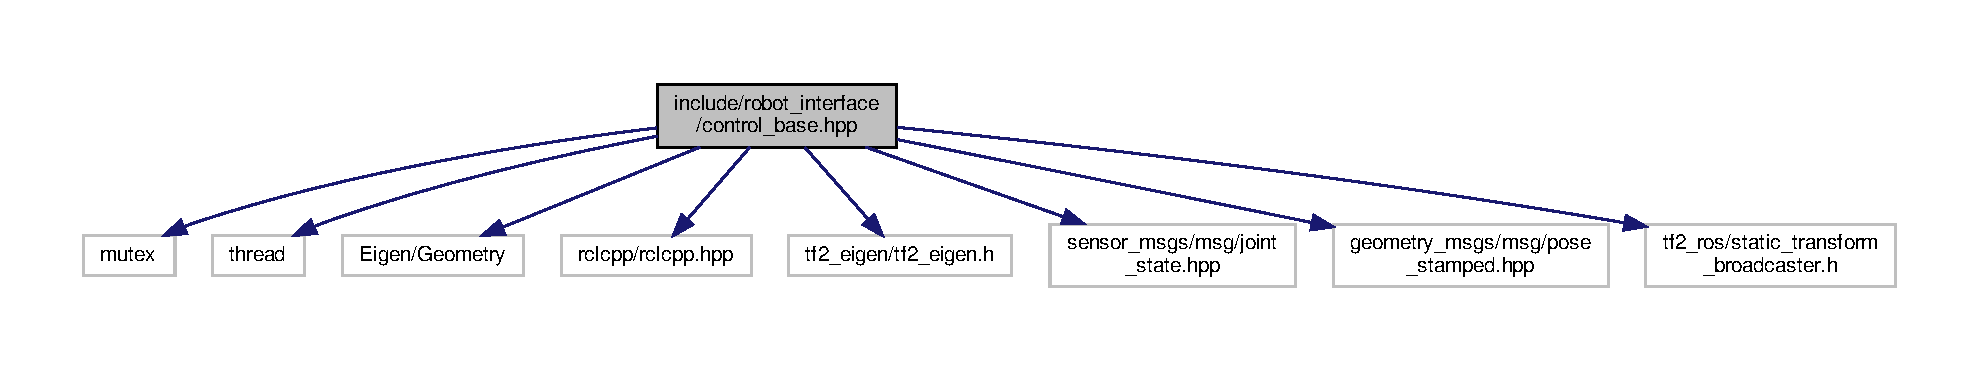
\includegraphics[width=350pt]{control__base_8hpp__incl}
\end{center}
\end{figure}
This graph shows which files directly or indirectly include this file\+:
\nopagebreak
\begin{figure}[H]
\begin{center}
\leavevmode
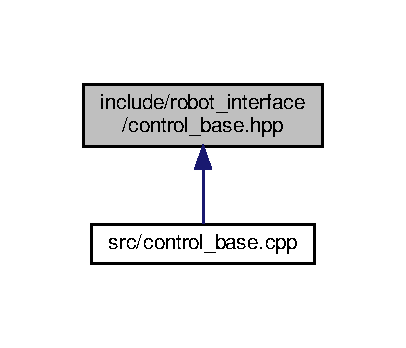
\includegraphics[width=195pt]{control__base_8hpp__dep__incl}
\end{center}
\end{figure}
\subsection*{Classes}
\begin{DoxyCompactItemize}
\item 
struct \hyperlink{structTcpPose}{Tcp\+Pose}
\begin{DoxyCompactList}\small\item\em Data type to represent robot arm\textquotesingle{}s end-\/effector pose in 3D cartesian space. \end{DoxyCompactList}\item 
class \hyperlink{classArmControlBase}{Arm\+Control\+Base}
\begin{DoxyCompactList}\small\item\em Robot arm control interface. \end{DoxyCompactList}\end{DoxyCompactItemize}


\subsection{Detailed Description}
Native robot control interface for visual manipulation. 

\begin{DoxyAuthor}{Author}
Yu Yan 
\end{DoxyAuthor}
\begin{DoxyDate}{Date}
29 Sep 2019 This file contains the control interface template to make the visual grasping. The interface is used for the control between a PC and an industrial robot controller. Collision detection is not considered in this interface. The specific behaviors are supposed to be filled with the communication protocal of an industrial robot, which are usually specified by the robot manufacturors. 
\end{DoxyDate}

\hypertarget{control__base_8cpp}{}\section{src/control\+\_\+base.cpp File Reference}
\label{control__base_8cpp}\index{src/control\+\_\+base.\+cpp@{src/control\+\_\+base.\+cpp}}
{\ttfamily \#include $<$robot\+\_\+interface/control\+\_\+base.\+hpp$>$}\newline
{\ttfamily \#include $<$chrono$>$}\newline
{\ttfamily \#include $<$thread$>$}\newline
Include dependency graph for control\+\_\+base.\+cpp\+:
\nopagebreak
\begin{figure}[H]
\begin{center}
\leavevmode
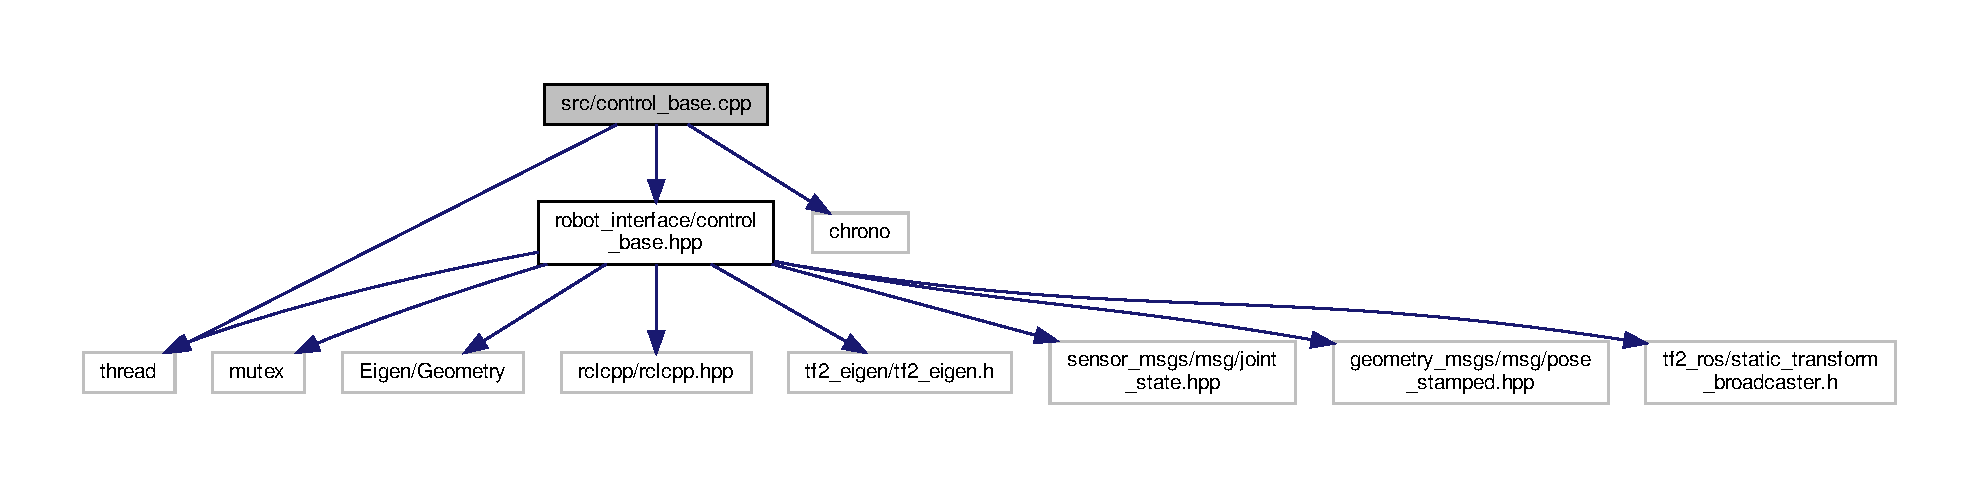
\includegraphics[width=350pt]{control__base_8cpp__incl}
\end{center}
\end{figure}

%--- End generated contents ---

% Index
\backmatter
\newpage
\phantomsection
\clearemptydoublepage
\addcontentsline{toc}{chapter}{Index}
\printindex

\end{document}
